
%%%%%%%%%%%%%%%%%%%%%%% file typeinst.tex %%%%%%%%%%%%%%%%%%%%%%%%%
%
% This is the LaTeX source for the instructions to authors using
% the LaTeX document class 'llncs.cls' for contributions to
% the Lecture Notes in Computer Sciences series.
% http://www.springer.com/lncs       Springer Heidelberg 2006/05/04
%
% It may be used as a template for your own input - copy it
% to a new file with a new name and use it as the basis
% for your article.
%
% NB: the document class 'llncs' has its own and detailed documentation, see
% ftp://ftp.springer.de/data/pubftp/pub/tex/latex/llncs/latex2e/llncsdoc.pdf
%
%%%%%%%%%%%%%%%%%%%%%%%%%%%%%%%%%%%%%%%%%%%%%%%%%%%%%%%%%%%%%%%%%%%


\documentclass[runningheads,a4paper]{llncs}

\usepackage{amssymb}
\setcounter{tocdepth}{3}
\usepackage{graphicx}
\usepackage{url}

\usepackage{amsmath} % assumes amsmath package installed
\usepackage{amssymb}  % assumes amsmath package installed
\renewcommand{\UrlFont}{\small\tt}
\usepackage{graphicx}
\usepackage{listings}
\usepackage{color}
\usepackage[tight]{subfigure}
\usepackage{balance}
\usepackage[ruled,vlined]{algorithm2e}
\usepackage{listings}
\usepackage{courier}


\urldef{\mailsa}\path|{jorgemunoz, imaza, fcaballero, aollero}@us.es|
\newcommand{\keywords}[1]{\par\addvspace\baselineskip
\noindent\keywordname\enspace\ignorespaces#1}

\begin{document}

\mainmatter  % start of an individual contribution

\graphicspath{{./}{./figures/}}

% first the title is needed
\title{Task allocation for teams of aerial robots equipped with manipulators in assembly operations}


% a short form should be given in case it is too long for the running head
\titlerunning{Task allocation for aerial robots in assembly operations}

% the name(s) of the author(s) follow(s) next
%
% NB: Chinese authors should write their first names(s) in front of
% their surnames. This ensures that the names appear correctly in
% the running heads and the author index.
%
\author{Jorge Munoz-Morera%
\and Ivan Maza\and Fernando Caballero\and Anibal Ollero
\thanks{This work has been partially supported by the ARCAS Project (FP7-ICT-287617) funded by the EU FP7 and the RANCOM (P11-TIC-7066) and AEROMAIN (DPI2014-59383-C2-1-R) national projects} % $<$-this % stops a space
}
%
\authorrunning{Task allocation for aerial robots in assembly operations}
% (feature abused for this document to repeat the title also on left hand pages)

% the affiliations are given next; don't give your e-mail address
% unless you accept that it will be published
\institute{Grupo de Rob\'{o}tica, Visi\'{o}n y Control, Universidad de Sevilla, Camino de los Descubrimientos s/n, 41092 Sevilla, Spain.
\mailsa
}

%
% NB: a more complex sample for affiliations and the mapping to the
% corresponding authors can be found in the file "llncs.dem"
% (search for the string "\mainmatter" where a contribution starts).
% "llncs.dem" accompanies the document class "llncs.cls".
%

\toctitle{Task allocation for aerial robots in assembly operations}
\tocauthor{J. Munoz-Morera, I. Maza, F. Caballero, A. Ollero}
\maketitle


\begin{abstract}
The work presented in this paper is part of the autonomous planning architecture of a team of aerial robots equipped with on-board robotic arms. The mission of the team is the construction of structures in places where the access is difficult by conventional means, which is the scenario considered in the framework of the ARCAS European Project. This paper presents a planning engine for this context. From the 3D CAD model of the structure an assembly planner computes the required assembly tasks, which are the inputs for the system. These tasks are assigned to the available aerial robots by a task allocation planner, which computes an assignment and improves it step by step by communicating with a symbolic planner. The latter estimates the cost of the sequence of actions needed in the mission execution for the given assignment. This paper presents simulation results that show the feasibility of the approach and a comparison between different solvers.
\keywords{Assembly Planning; Symbolic Planning; Task Planning; Task Allocation; Multiple Aerial Robots}
\end{abstract}

\section{Introduction and Related Work}
\label{sec:intro}

The work described in this paper is part of the ARCAS European Project~\cite{kondak_ijars13} funded by the European Commission. One of the goals of this project is to build a structure by using a team of aerial robots equipped with on-board manipulators. The practical interest of this system can be found in situations where it is required to build a structure in places with difficult access by conventional means.

Although Unmanned Aerial Systems (UAS) have been designed and developed for performing military missions, currently the trend is to extend their applicability to civil mission such as firefighting, critical infrastructure protection or remote surveillance, among many others.  The multiple variety of platforms, control systems and ground-based equipments~\cite{perez_jint13,maza_jint10_multimodal}, and the heterogeneity of the communication devices have made difficult the interoperability among different systems. 

Several works~\cite{maza_icuas14,maza_jfr11_multiuav} have addressed cooperation in teams of aerial robots for multi-purpose missions. However, in those papers the dexterous manipulation with aerial robots was not present. The use of aerial robots allows to perform assembly tasks in any point of the 3D space, which can represent a relevant advantage compared to ground robots in areas of difficult access.

%Assembly planning is the process of creating a detailed assembly plan to craft a whole product from separate parts by taking into account the final product geometry, available resources to manufacture that product, fixture design, feeder and tool descriptions, etc. Efficient assembly plans can reduce time and costs significantly. The assembly planning problem has been shown to be an NP-complete problem~\cite{Kavraki93} and covers three main assembly subproblems: sequence planning, line balancing, and path planning. Reference~\cite{Jimenez2011} presents a survey on assembly sequencing from a combinatorial and geometrical perspective.

Most existing classical planners can be classified into two categories~\cite{ingrand_ghallab_2013}: planners which use domain-dependent knowledge and planners which use domain-independent knowledge. The former can exploit their specific knowledge to guide the planning process and solve larger problems faster than other planners, with the disadvantage of needing a person who gives the knowledge on how to solve the problems. Such knowledge can be designed using temporal logic (TLPlan~\cite{Bacchus00usingtemporal} and TALplanner~\cite{Kvarnstrom01talplanner}) or task decomposition (SHOP2~\cite{Nau03shop2}, SIPE-2~\cite{Wilkins}, O-PLAN~\cite{Currie90}). On the other hand, a planner that uses domain-independent knowledge (SGPlan~\cite{Chen06}, FastDownward~\cite{Helmert06}, LPG~\cite{Gerevini01}) does not need specific knowledge so the domain formalization is simpler, with the disadvantage that the performance of the planner may be lower than that of domain-dependent planners. The integration of both types of planners, which let use their advantages and avoid their disadvantages, is a matter of study, and some works in that direction can be read in~\cite{Gerevini02} and~\cite{Shivashankar}.

%Below the task planning is situated the motion and manipulation planning, which should take into account the geometry, kinematics and dynamics of the problem. For motion planning there are consolidated techniques which produce very good results, such these based on Rapidly-exploring Random Trees~\cite{LaValle04}. Combined task and motion planning have been studied in different works~\cite{Cambon01012009,Wolfe,Lagriffoul01122014}, but this work only addresses up to task planning. A system on which teams of quadrotors assemble a 2.5-D structure from simple parts can be found in~\cite{Lindsey-RSS-11}. In that work the robots were equipped with grippers and the structure was supposed to be assembled sequentially, so no manipulation planning was done after picking the parts and the assembly tasks were not parallelizable.

This paper presents a planning engine to solve a general structure assembly problem with a team of aerial robots. This problem is formally presented in Sect.~\ref{sec:pdef}. From the 3D CAD model of the structure the assembly planner presented in Sect.~\ref{sec:assembly_symbolic} computes the required assembly tasks. These tasks are assigned to the available aerial robots by the task allocation planner described in Sect.~\ref{sec:tap}. This planner optimizes the computed assignment by calling the symbolic planner explained in Sect.~\ref{sec:assembly_symbolic}, which estimates the cost of the sequence of actions needed in the mission execution for the given assignment and gives feedback to the task allocation planner in the search of a better assignment. Section~\ref{sec:score_calc} explains with more detail the connection between the task allocation planner and the symbolic planner. Section~\ref{sec:results} includes simulation results that show the feasibility of the approach and a comparison between different solver configurations. Section~\ref{sec:conclusions} closes the paper with the conclusions and future work.

\section{Problem Statement}
    \label{sec:pdef}
    
Let us consider a mission $\mathcal{M}$ consisting on the assembly of a structure composed by several parts initially located around the environment. The parts have to be assembled on specific locations by a team of $n$ aerial robots starting the mission from their home locations. Then the mission is composed by a set of assembly tasks $\mathcal{T}$. Each of the parts has a weight and a dependency list consisting on the tasks that must be done prior to its assembly. Let us define $\mathcal{L}$ as the set of stock parts locations, $\mathcal{L'}$ as the set of locations where the parts have to be assembled and $\mathcal{H}$ as the home locations of the aerial robots. The objective is to assemble all the parts on their locations minimizing the travel flight times of the vehicles and exploiting the potential parallelism that can be achieved using multiple aerial robots.
    
The implicit combinatorial problem can be expressed by the edges of a graph $G(V,E)$ considering the following notation:
    
    \begin{itemize}
    	\item $\mathcal{T} = \{t_1, t_2, ..., t_m\}$ is a set of $m$ assembly tasks.
    	\item ${P_{i}} \subseteq \mathcal{T}  $ is the set of preconditions for the $i$-th task, i.e. the subset of tasks that must have been done prior to the execution of that task.
    	\item $n$ is the number of aerial robots.
    	\item $\mathcal{L} = \{l_1, l_2, ..., l_m\}$ is the set of stock parts locations and $\mathcal{L'} = \{l'_1, l'_2, ..., l'_m\}$ is the set of final assembly locations.    
    	\item $\mathcal{H} = \{h_1, h_2, ..., h_n\}$ is the set of aerial robots home locations.
  		\item $V=\{\mathcal{L}\cup\mathcal{L'}\cup\mathcal{H}\}=\{v_1, v_2, ..., v_{2m+n}\}$ is the set of vertices of the $G$ graph.
		\item $E=\{(v_i,v_j) | v_i,v_j \in V; i<j\}$ is the edge set.  		
  		\item ${R_{k} = \{r_1, r_2, ..., r_s} \}\subseteq$ $V$ is the route for the $k$-th aerial robot, composed by a subset of $s$ vertices from $V$.
		\item Cost $c_{r_i,r_j}$ is a non-negative travel time between vertex $r_i$ and $r_j$, where $c_{r_i,r_j}=c_{r_j,r_i}$.
		\item $p = \{p_1, p_2, ..., p_n\}$ is a vector with the maximum payloads of the aerial robots.
		\item $w = \{w_1, w_2, ..., w_m\}$ is a vector containing the weights of the parts.
		\item $q = \{q_1, q_2, ..., q_m\}$ is a vector containing the times on which the parts are finally assembled.
	\end{itemize}
	
The problem consists in determining a set $\mathcal{R}$ of routes with minimal cost and a vector $q$ of minimal task assembly times, with each route starting at the home locations of the vehicles, such that every vertex in $\mathcal{L}$ is visited at least by one vehicle and followed by its subsequent vertex in $\mathcal{L'}$, without exceeding the payload of each vehicle and respecting the preconditions for each of the parts. The possibility of visiting the same location with multiple aerial robots is given by the fact that some parts should be carried cooperatively by more than one aerial robot if they are too heavy. The problem described is similar to the well-known Vehicle Routing Problem (VRP)~\cite{Dantzig_Ramser_VRP}.	
	For the $k$-th aerial robot, the cost of a route is given by 

 \begin{equation}
 	{C(R_{k}) = \sum_{i=1}^{s-1} c_{r_i,r_{i+1}}} \, ,
 	\label{eq:route_cost}
 \end{equation}	

\noindent where ${r_1 \in \mathcal{H}}$, ${r_i \in V}$ and ${r_j \in}$ $\mathcal{L}$ ${\implies r_{j+1} \in}$ $\mathcal{L'}$. Considering that up to two aerial robots can cooperatively transport a single heavy part, this route ${R_{k}}$ is feasible if ${(p_k \geq w_j) \lor (\exists R_{z} | r_j \in R_{z} \land (p_k+p_z) \geq w_j)}$, i.e. the weight of each part does not exceed the maximum payload of the aerial robot transporting it or there is another available aerial robots so that both can transport it cooperatively. For each part $w_j$ in this route it must be met in addition that $\forall t_{s} \in P_{j}: q_{s}<q_{j}$, i.e. all the parts from its set of preconditions must have been assembled before that part.
	
The goal of the planner is to minimize the total travel time $\sum_{i=1}^{n} C(R_{i})$ of the feasible routes executing all the assembly tasks of the mission and balance the workload of the different aerial robots.

\section{Assembly and Symbolic Planners}
	\label{sec:assembly_symbolic}

The input for the planning engine is the 3D CAD model of the structure that has to be build. This model is loaded by the assembly planner, whose purpose is to obtain an assembly plan with all the assembly tasks needed to build the structure. The assembly plan is computed by using the \emph{assembly-by-disassembly} technique, consisting on finding a plan to disassemble the whole structure and reversing the order of its operations to get the final assembly plan. In that plan, each task represents the assembly of one specific part of the structure and contains the preconditions that must be met prior to its execution, namely the assembly tasks that must be done before the assembly of that specific part. The only requirement to execute an assembly task from the plan is to have its preconditions met. That feature makes the computed assembly plan totally independent on the number of vehicles available for its execution.

Some of the tasks in the computed assembly plan could be executed in parallel to reduce the whole mission assembly time. This information is implicitly encoded in the plan as the tasks preconditions. At any given moment, all the assembly tasks that have their preconditions met could be executed in parallel. In addition to the minimization of the assembly time, a low level plan must be computed for each aerial robot. Feasible paths must be computed for the navigation of the robots, both for the part picking and the part assembling. Also, those assembly tasks that must be executed cooperatively between robots require synchronization among the involved aerial robots. 

In this paper, the JSHOP2 symbolic planner~\cite{Nau03shop2} has been applied to order the assembly tasks and compute a low level plan for each aerial robot. JSHOP2 is a domain-independent planning system based on Hierarchical Task Networks (HTN) that decomposes the tasks into smaller subtasks and so on, until obtaining low-level tasks that can not be further decomposed and thus can be directly performed. An assembly domain has been designed for the JSHOP2 symbolic planner, which receives the assembly plan and computes an ordering of the assembly tasks, as well as low-level plans for each of the involved aerial robots. To compute the low-level plans, the symbolic planner needs an assignment of assembly tasks to aerial robots which is in turn computed by the task allocation planner presented in the next section. After computing the low-level plans the symbolic planner makes a cost estimation for the execution, whose value will be used by the task allocation planner to try to find a better assignment.

A more detailed description for the assembly and the symbolic planners can be found in~\cite{munoz_icuas15}.

\section{Task Allocation Planner}
    \label{sec:tap} 

The planner chosen to solve the assignment problem presented in Sect.~\ref{sec:pdef} was OptaPlanner~\cite{optaplanner}, an open source, multi-platform planning engine written in Java and released under Apache Software License. OptaPlanner is aimed to solve planning problems with resource usage optimization. It is capable of generating near-optimal plans by applying optimization heuristics and meta-heuristics combined with score calculation. One of his main advantages is that the solver's algorithm is highly configurable. In OptaPlanner it is possible to use different heuristics and meta-heuristics algorithms applied in sequence, so that the user can select the most suitable for the problem in question. The optimization is done in base of a score calculation that is computed after all the planning entities have been assigned. This score determines the suitability of the last computed solution: if after searching for a new solution the new score is worse than the score calculated in the previous solution, then the last solution is discarded and the process continues trying to generate a solution with a better score.

\subsection{Problem Domain}
    \label{sec:optaplanner_domain}

In OptaPlanner the entities of the real world that must be assigned are called \emph{planning entities}, and are represented as Java classes. These planning entities have one or more \emph{planning variables}, represented as Java attributes that take different \emph{planning values} over the planning process. To solve an assignment problem, each of the planning entities must have been given a valid planning value for each of its planning variables.

For the problem defined in this section the domain has been defined as follow: the planning entities are the assembly tasks. Each assembly task represents a part that is stored on a specific location and that must be assembled on a certain location by an aerial robot. Each assembly task has defined a chained planning variable. This chained planning variable takes as value the assembly task that has been assigned before the actual. All chains start from the positions where the aerial robots are landed, so the first assigned task will allways point to an aerial robot, the second assigned task will point to the first assigned task or to another aerial robot, and so on. By this way when all planning entities have been assigned, those that are present in the same chain are considered to be assigned to the same aerial robot. 

\subsection{Solver Phases}
    \label{sec:solver_phases}

As it was mentioned before, the OptaPlanner solver can use multiple optimization algorithms in sequence. Each of the optimization algorithms used is called a solver phase. During the execution of the solver there is never more than one solver phase executing at the same time, so a solver phase only starts when the previous phase has finished. There are three types of solver phases that can be used in the OptaPlanner solver: Construction Heuristics (CH), Metaheuristics (MH) and Exhaustive Search (ES). 

The CH solver phase builds an initial solution in a short time. The solution computed is not always feasible, but it tries to find it fast so that the following solver phases can finish the search of a feasible one by starting from that initial solution. There are different algorithms that can be used as CH. One common characteristic of them is that when a CH assigns a planning entity, that assignment remains unchanged until the end of the algorithm. This is the main reason that makes the CH algorithms find solutions that may be unfeasible: no re-planning is done at this phase.

The MH solver phase is based on different types of local search algorithms. Local search starts from the initial solution computed by the CH phase and evolves it into a mostly better and better solution. At each solution, it evaluates a number of moves between the planning entities and applies the most suitable to step to the next solution, whose score may be better, equal or worse than the previous. Allowing as solution a new one which has a worse score than the previous is important because it avoids getting stuck in local minima. Another important thing to be taken into account is that the local search does not use a search tree, but a search path. When finding a new solution all possible moves are evaluated but unless it is the chosen move, it does not investigate further the rest of possible solutions. That makes the local search very scalable, but as a disadvantage it may not find never the optimal solution.

Finally, the ES solver phase does not depend on previous phases and it is applied alone. Brute force or the branch and bound algorithms are available. These methods guarantee the find of the optimal solution for a problem, but are poorly scalable so are not usually chosen to solve real problems.

\subsection{Solution Moves}
    \label{sec:sol_moves}
    
To create a new solution the solver generates all moves that is possible to do from the last solution and selects a subset of them to be evaluated. A move is a change in the value of a planning variable for one or more planing entities, which results in a new assignment. From the selected subset of moves the solver chooses the one which produces the better score and applies it to the current solution to generate a new one. The chosen move is called step.

The solver can be configured to use multiple classes that allow to do different types of moves among the planning entities, called selectors. It is possible to use any of the available selectors on any problem domain, although the suitability of the selectors depends on the problem type. The most common selectors used in different problem types (Fig.~\ref{fig:moves}) are the following:

    \begin{itemize}
    		\item Change move: selects one planning entity and modify the value of its planning variable.
    		\item Swap move: selects two planning entities and swap the value of its planning variables.
    		\item Subchain Change move: selects a subchain of planning entities and moves them to a different chain or to a different position inside the same chain where they were selected.
    		\item Subchain Swap move: selects two subchains of planning entities from different chains or from the same chain and swaps its positions.
	\end{itemize}
	
	\begin{figure}
    		\centering
    		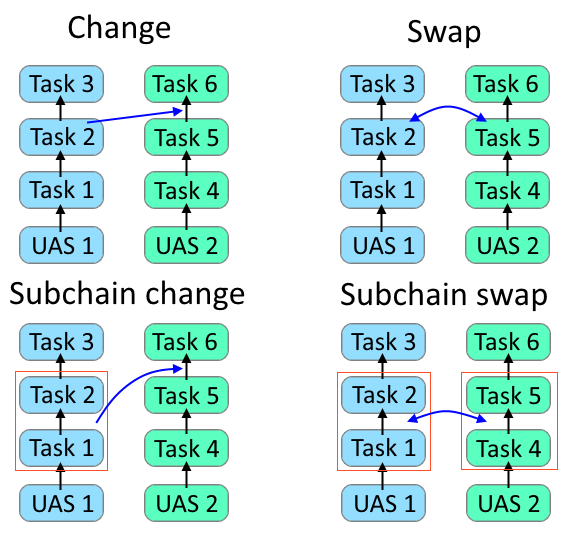
\includegraphics[width=0.4\columnwidth]{moves.png}
    		\caption[Effects of the Move, Swap, Subchain Move and Subchain Swap selectors.]{Effects of the Move, Swap, Subchain Move and Subchain Swap selectors over two different chains of planning entities.}
    		\label{fig:moves}
	\end{figure}
	
Over the selectors is possible to apply filters. A filter is a condition that is checked over each of the moves generated by the selector. If the move does not meet the condition it is then discarded and another different move is generated again, until obtaining a valid one. With this mechanism is possible to discard early those moves that are known to produce a bad score before being evaluated by the solver, saving computation time and better assisting the search of the solution.

\section{Connecting the Task Allocation Planner and Symbolic Planner}
    \label{sec:score_calc}

To compare the suitability of the different solutions computed along the task allocation process, a score-based calculation is done after each new solution is found. This score is based on the definition of three types of constraints with different levels of relevance. Given a new solution, its score consists on the sum of the broken constraints for each of the constraint types defined for the problem. The constraint types are:

    \begin{itemize}
    	\item Hard-constraints: these are constraints that must not be broken in any case. A broken hard-constraint will lead to an unfeasible plan, so its sum must be zero. The hard-constraints defined for the assembly problem say that the weight of a part must not exceed the payload capability of the aerial robot it has been assigned to.
    	\item Medium-constraints: these are constraints that are desirable to be broken the less as possible. Its importance is under the importance of the hard-constraints but above the importance of the soft-constraints. The one defined measures the potential parallelism that can be achieved with the current assignment, desired to be as high as possible.
    	\item Soft-constraints: these are the constraints with lower priority. They have the lowest impact when broken, but still they must be minimized. The soft-constraint defined tries to minimize the distance travelled by all the aerial robots.
	\end{itemize}
	
After a new solution is found, the score related to the new assignment is calculated. The sums that come from the hard and medium constraints can be computed from inside the task allocation planner. However that is not the case for the soft-constraints, as they measure the distance travelled by the aerial robots during the assembly. That distance can only be estimated if the order of the assembly operations is previously known, but as commented in Sect.~\ref{sec:assembly_symbolic} this order is not specified explicitly in the assembly plan. To solve this, the assignment computed by the task allocation planner is given as input to the symbolic planner. The symbolic planner computes an order for the assembly tasks and gives an estimation of the distance travelled by the aerial robots during the assembly for the given assignment. This estimation is returned to the task allocation planner, which uses it as the soft-constraint value closing the score calculation loop. 

By this way, the optimization of the assignment is done cooperatively between the task allocation planner and the symbolic planner while preserving each of them its own domain.

\section{Simulation Results}
\label{sec:results}

In this section a representative mission will be used to measure the plan quality and computation times of the whole planning engine comparing different solver configurations. In this mission, a fleet composed of four aerial robots equipped with robotic arms is used. The environment contains twenty-six locations of interest (see Fig.~\ref{fig:environment}) where eleven of them are the initial locations for the parts, another eleven are the assembly locations and four are home locations for the aerial robots. The mission is composed by eleven assembly tasks corresponding to the eleven parts that conform the structure. 

\begin{figure}
    \centering
    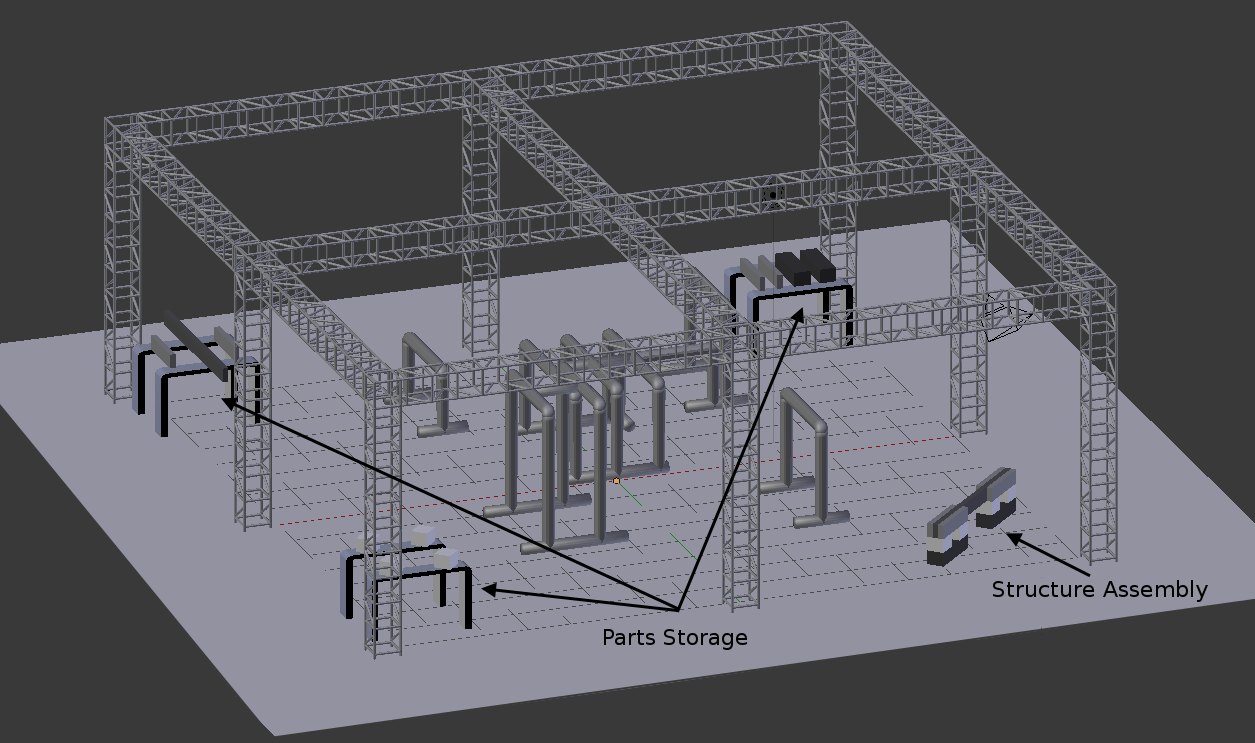
\includegraphics[width=0.75\columnwidth]{final_scene.png}
    \caption[Environment modelled for the mission.]{Environment modelled for the mission. The parts are initially stored over tables in three different stock areas and finally assembled in the lower right corner of this figure.}
    \label{fig:environment}
\end{figure}

The workflow of the planning engine is as follows: the entry point to the system is the 3D CAD environment model that contains the initial state (stock parts and home locations of the aerial robots) and the 3D CAD model of the structure to be built. The assembly planner reads the 3D CAD model of the structure and generates a valid assembly plan. Given the assembly plan, the task allocation planner solves the assignment problem and tries to optimize it by communicating with the symbolic planner, which in turn finds a low-level plan for each of the aerial robots and returns a cost that is used by the task allocation planner in the optimization process.

The baseline solver configuration has the following features:

\begin{itemize}
  \item One Construction Heuristic solver phase, configured with a First Fit Decreasing algorithm. This algorithm sorts the planning entities by decreasing difficulty and assigns the planning entity which produces the best score at each time, until no left are unassigned.
  \item One Local Search solver phase, configured with a Late Acceptance algorithm. This algorithm tries to optimize the assignment by doing one move and accepting it if does not decrease the score or leads to a score that is at least the score of a fixed number of steps ago.
  \item Four different move selectors, included inside a fifth union selector that selects with the same probability at each step one of the others to generate the next move.
\end{itemize}

From the baseline solver configuration template, a total of seven new solver configurations were created to test them against the former. All of them have been created with exactly the same Construction Heuristic and Local Search algorithm as the baseline, as well as the same move selectors, but differ in two main characteristics. The first is that all the new configurations have the sub-chain move selectors to discard as moves the reverse of a given selected sub-chain, reducing thus the number of possible moves to do between steps. The second is that a filter has been specifically implemented for each of the new configurations to try to discard moves that are known to produce bad scores and that lead to a waste of computation time. So, the main difference among the baseline configuration and the test configuration are the use of filters.

The descriptions of the solver configurations used in the simulation besides the baseline are the following:

\begin{itemize}
  \item Late Acceptance Change Filter: a filter is defined to avoid moving a planning entity from a position in a chain to another position in the same chain. This is because the order of the planning entities inside the same chain is finally computed by the symbolic planner and not by the task allocation planner, and thus these moves are redundant because will all produce the same score.
  \item Late Acceptance Swap Filter: a filter is defined to avoid swapping planning entities from the same chain.
  \item Late Acceptance ChangeSwap Filter: a combination of the two previous filters.
  \item Late Acceptance SubChainChange Filter: a filter is defined to avoid moving a sub-chain of planning entities from a position in a chain to another position in the same chain.
  \item Late Acceptance SubChainSwap Filter: a filter is defined to avoid swapping sub-chains of planning entities from the same chain.
  \item Late Acceptance Nearby Filter: this configuration tries to make moves among those planning entities that are near each other in distance terms, to try to minimize the travelled distance.
  \item Late Acceptance NearbyCS Filter: a combination of the previous filter and the ChangeSwap filter.
\end{itemize}

The score and performance results obtained after running the simulation for each of the eight solver configurations can be seen on Table~\ref{table:score}. The solver configuration that achieved the best score was the ChangeSwap Filter configuration, improving the score obtained by the default configuration in 19 units for the Soft constraints. 

With respect the average calculate count per second, which measures how fast the solver is, the ChangeSwap Filter configuration achieved again the highest ratio, doing two times the score calculate count per second achieved by the default configuration. The two configurations that used the nearby technique achieved the worst values, obtaining only one per second.

\begin{table}
	\begin{center}
		\begin{tabular}{ | l | c | c | c | c |}
	\hline
   Solver & Hard & Medium & Soft & Score computation rate\\ \hline
   ChangeSwap Filter & 0 & 0 & -320 & 6/s \\ \hline
   Swap Filter & 0 & 0 & -329 & 2/s \\ \hline
   SubChainChange Filter & 0 & 0 & -330 & 2/s \\ \hline
   Change Filter & 0 & 0 & -338 & 5/s \\ \hline
   SubChainSwap Filter & 0 & 0 & -338 & 2/s \\ \hline
   Default & 0 & 0 & -339 & 3/s \\ \hline
   Nearby Filter & 0 & 0 & -339 & 1/s \\ \hline
   Nearby CS Filter & 0 & -1 & -358 & 1/s \\ \hline
		\end{tabular}
	\end{center}
	\caption{Simulation results for each of the solvers, obtained for the example mission. The Hard, Medium and Soft columns show the sum of the broken constraints for each constraint type, given as negative values. The score computation rate is the average score calculation count per second for each solver configuration. The simulation was run on a machine with an Intel i7 CPU at 2 GHz and 8GB RAM.}
	\label{table:score}
\end{table}

Figure~\ref{fig:sim2} show a screenshot of the mission execution during the simulation.

%\begin{figure}
%    \centering
%    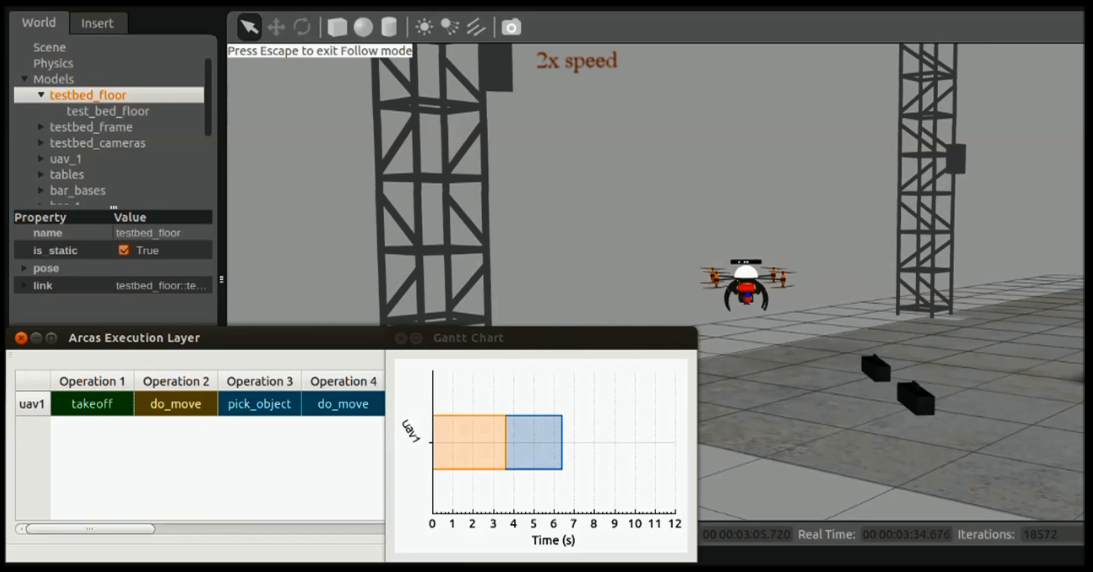
\includegraphics[width=0.8\columnwidth]{sim1.png}
%    \caption[Simulation screenshot of a takeoff action.]{Simulation screenshot of a takeoff action done by an aerial robot in the example mission execution for the planning framework. A visualization tool shows the state of each of the actions present in the plan as well as a Gantt chart of the mission execution.}
%    \label{fig:sim1}
%\end{figure}

\begin{figure}
    \centering
    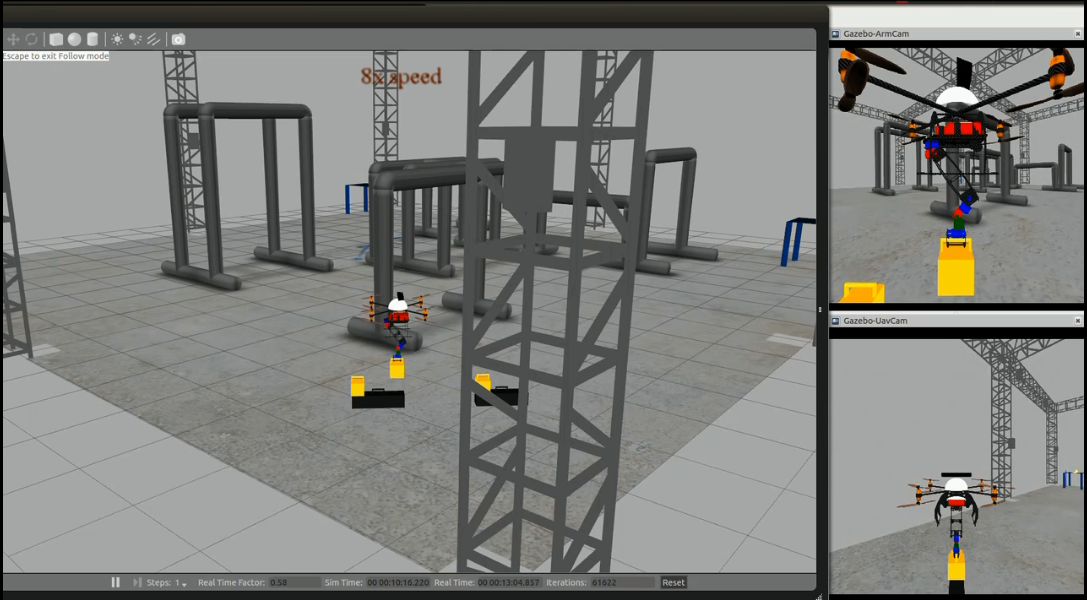
\includegraphics[width=0.75\columnwidth]{sim3.png}
    \caption[Simulation screenshot of an assembly action.]{Simulation screenshot of an assembly action done by an aerial robot. All parts have a handle from which the aerial robots can take them and a cavity beneath that let them be stacked. A video of the mission can be downloaded from \url{http://grvc.us.es/robot2015plan}.}
    \label{fig:sim2}
\end{figure}

\section{Conclusions and Future Work}
	\label{sec:conclusions}

The system developed performs task assignment and scheduling given the number of aerial robots in order to increase the parallelism and cooperation in the mission. The main contribution of the paper is the successful connection of the task allocation planner with the symbolic planner in the context of structure assembly missions.

However the approach has been tested in missions involving multiple simulated aerial robots. In future work the goal is to execute the mission with real aerial robots in order to find more realistic and complex contexts to test the architecture developed.

%-----------------------------------------------------------------------------
% BIBLIOGRAPHY
%-----------------------------------------------------------------------------
\bibliographystyle{IEEEtran}
\bibliography{IEEEabrv,bibliography}

\end{document}
